\documentclass[9pt]{beamer}

\usepackage{graphicx}
\mode<presentation>
{
  \usetheme{Antibes}
  \setbeamercovered{transparent}
}


\usetheme{CambridgeUS}
\usecolortheme{default}
\usefonttheme{default}
\usefonttheme{structurebold}
\setbeamertemplate{enumerate items}[]

\usepackage[english]{babel}
\usepackage[latin1]{inputenc}
\usepackage{times}
\usepackage[T1]{fontenc}
\usepackage{Sweave}
\usepackage{ragged2e}
\usepackage{amsmath}
\usepackage{amssymb}
\usepackage{amsthm}
\usepackage{color}
\usepackage{booktabs}
\usepackage{tabularx}
\usepackage{hyperref}
\usepackage{graphicx}
\usepackage{color, colortbl}
\usepackage[date=iso8601, urldate=iso8601, style=verbose,
bibencoding=utf8, natbib=true, backend=biber]{biblatex}


\title{Impact of regulatory intervention on FPI
  bond-holding patterns}
\author{Finance Research Group, IGIDR}

\newcommand{\thedate}{\today}
\date{\thedate}

\begin{document}

\setbeamertemplate{headline}
{
  \leavevmode
                    \hbox{
                      \begin{beamercolorbox}[wd=0.4925\paperwidth, ht=2.25ex, dp=1ex, center]{title in head/foot}
                        \usebeamerfont{title in head/foot}\insertshorttitle\hspace*{3em}
                      \end{beamercolorbox}
                      \begin{beamercolorbox}[wd=0.4925\paperwidth, ht=2.25ex, dp=1ex, center]{section in head/foot}
                        \usebeamerfont{section in head/foot}\insertsection\hspace*{3em}
                      \end{beamercolorbox}
                    }
                    \vskip0pt
                  }

\setbeamertemplate{footline}
                  {
                    \leavevmode
                    \hbox{
                      \begin{beamercolorbox}[wd=0.35\paperwidth, ht=2.25ex, dp=1ex, center]{author in head/foot}
                        \usebeamerfont{author in head/foot}\insertshortauthor\hspace*{3em}
                      \end{beamercolorbox}
                      \begin{beamercolorbox}[wd=0.281\paperwidth, ht=2.25ex, dp=1ex, center]{date in head/foot}
                        \usebeamerfont{date in head/foot}\insertshortdate\hspace*{3em}
                        \insertframenumber{} / \inserttotalframenumber\hspace*{1ex}
                      \end{beamercolorbox}
                      \begin{beamercolorbox}[wd=0.35\paperwidth, ht=2.25ex, dp=1ex, right]{institute in head/foot}
                        \usebeamerfont{institute in head/foot}\insertinstitute\hspace*{3em}
                      \end{beamercolorbox}
                    }
                    \vskip0pt
                  }
                    

% \setbeamercolor{item projected}{bg=red}
% \setbeamercolor{subitem projected}{bg=red}
\setbeamertemplate{itemize item}[triangle]
\setbeamertemplate{itemize subitem}[square]
\setbeamercolor{itemize item}{fg=darkred}
\setbeamercolor{itemize subitemitem}{fg=darkred}
%\setbeamercolor{enumerate projected}{fg=darkred}
%\setbeamercolor{enumerate subitemitem}{fg=darkred}

\newcommand{\hi}[1]{\textcolor{red}{#1}}

\newcommand{\fullpage}[1]{
  \part{#1}
  \begin{frame}
    \partpage
  \end{frame}
}


\addtocounter{framenumber}{-1}
{
  \setbeamertemplate{headline}{}
  \setbeamertemplate{footline}{}
  \begin{frame}
    \titlepage
  \end{frame}
}
 
%% \newcommand{\presenter}{
%%   \centering \textit{\ Presented by Anurag Dutt (FRG, IGIDR)}
%% }

\begin{frame} \frametitle{Objective} 
  To analyse change in bond holding
  patterns around a regulatory intervention by the RBI.
\end{frame}


\begin{frame}
  \frametitle{The regulatory intervention} 
  In the RBI and SEBI circulars dated, 3rd Feb 2016, the following restrictions were
  imposed:
  \begin{itemize}
  \item All future investments by FPIs within the USD 51 bn Corporate
    Debt limit category, shall be required to be made in corporate bonds
    with a minimum residual maturity of three years.
  \item Consequently, FPIs shall not be allowed to make any
    further investment in CPs.
  \item No investments in debt secuities with optionality clause
    exercisable within three years, shall be made by FPIs.
  \item They shall not be permitted to invest in liquid and money
    market mutual fund schemes.
  \item However, there will be no lock-in period and FPIs shall be free to sell
    the securities (including those that are presently held with less than
    three years residual maturity) to domestic investors.
  \item This circular shall come into effect immediately.
  \end{itemize}  
\end{frame}


\begin{frame}
  \frametitle{Stated rationale}
  The only rationale stated in the 6th Bi-Monthly Monetary Policy
  Statement, released 3rd February is:\\
  \begin{enumerate}
  \item \textit{To harmonize requirements for investments by FPIs across
      both Government securities markets and corporate bond markets,}
  \end{enumerate}
\end{frame}



\begin{frame}
  \frametitle{Anticipated consequences}
  As a consequence of the regulation, FPIs could:\\
  \begin{itemize}
  \item Take money out of Indian CoBo markets, due to abrupt changes
    in investment guidelines.
  \item Or as  desired, switch from short-term to long-term CoBos.  
  \end{itemize}
  Standing 1 year 8 months from the date of notification of the
  circular, we analyse trends in FPI holdings of securities, to
  substantiate the real impact of the regulation. 
\end{frame}




\fullpage{Analysis of trends in FPI transactions: pre-post RBI intervention}
\section{Analysis of trends in FPI transactions: pre-post RBI intervention}


\begin{frame}
  \frametitle{Data}
  \begin{itemize}
  \item FPI and FII holdings from 01-01-2015 to 20-03-2016 are
    analysed.
  \item We aggregate multiple accounts under same PAN ID.
  \item Only Individual and corporate Foreign portfolio investors and
    FIIs are subsetted.
  \item List of long and short term bonds and commercial papers are
    taken from NSDL archives.
  \item For the purpose of analysis, we remove FPI accounts which have
    not held a single bond in the entire period of analysis.
 
  \end{itemize}
\end{frame}

\fullpage{Results}
\section{Results}

%%%%%%%%%%%%%%%%%%%%%%%%%%%%%%%%%%%%%%%%%%%%%%%%%%%%%%%%%%%%%%%%%%%%%%%%%%%%%%%%%%%%%%%%%%%%%%%%%%%%%%%%%%%%
% \begin{frame}                                                                                            %
%  \frametitle{All unique corporate bond ISINs - Median}                                                   %
%    \centering                                                                                            %
%    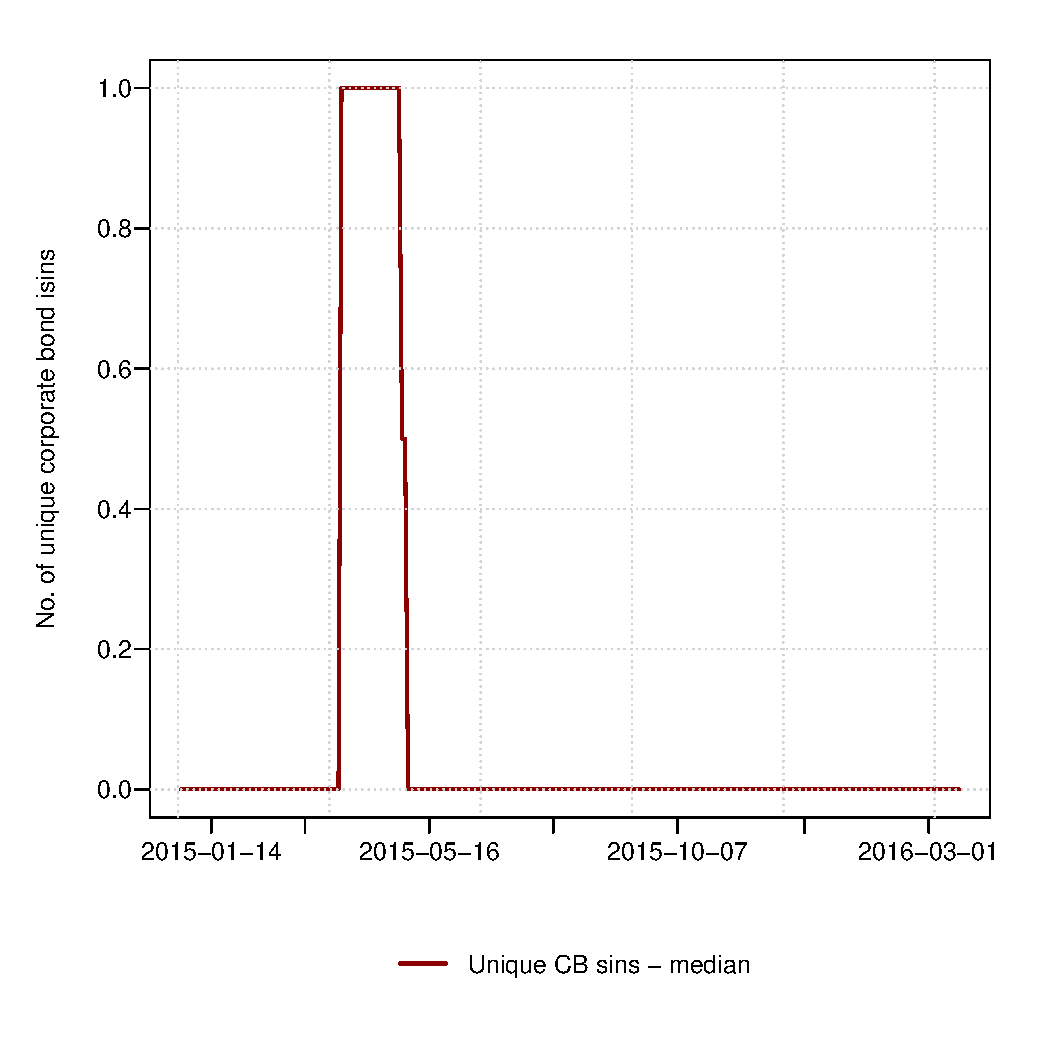
\includegraphics[width=0.8\paperwidth,height=0.5\paperwidth]{../GRAPHS/fpi_median_all_cbs_all.pdf}    %
% \end{frame}                                                                                              %
%                                                                                                          %
% \begin{frame}                                                                                            %
%  \frametitle{Unique long term corporate bond ISINs - Median}                                             %
%    \centering                                                                                            %
%    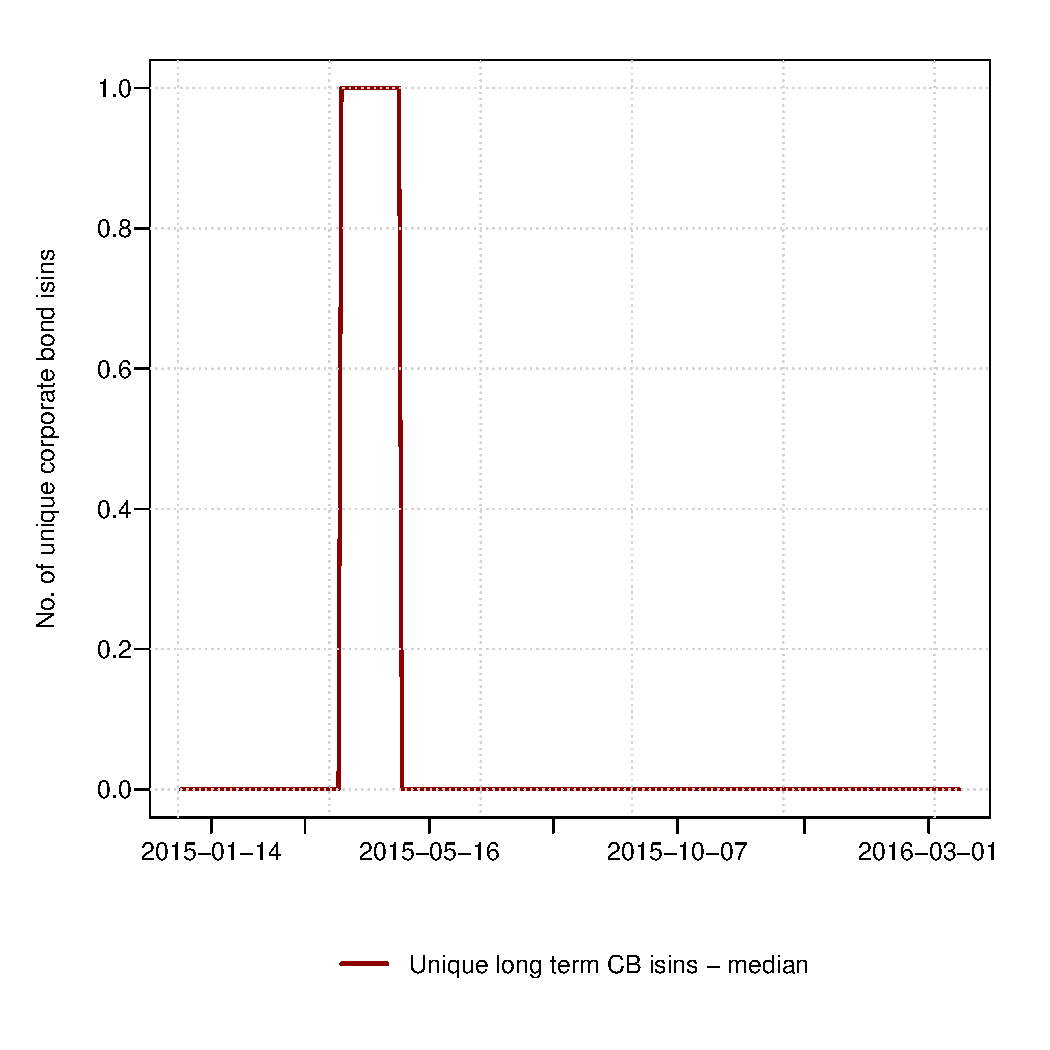
\includegraphics[width=0.8\paperwidth,height=0.5\paperwidth]{../GRAPHS/fpi_median_lt_cbs_all.pdf}     %
% \end{frame}                                                                                              %
%                                                                                                          %
% \begin{frame}                                                                                            %
%  \frametitle{Unique short term corporate bond ISINs - Median}                                            %
%    \centering                                                                                            %
%    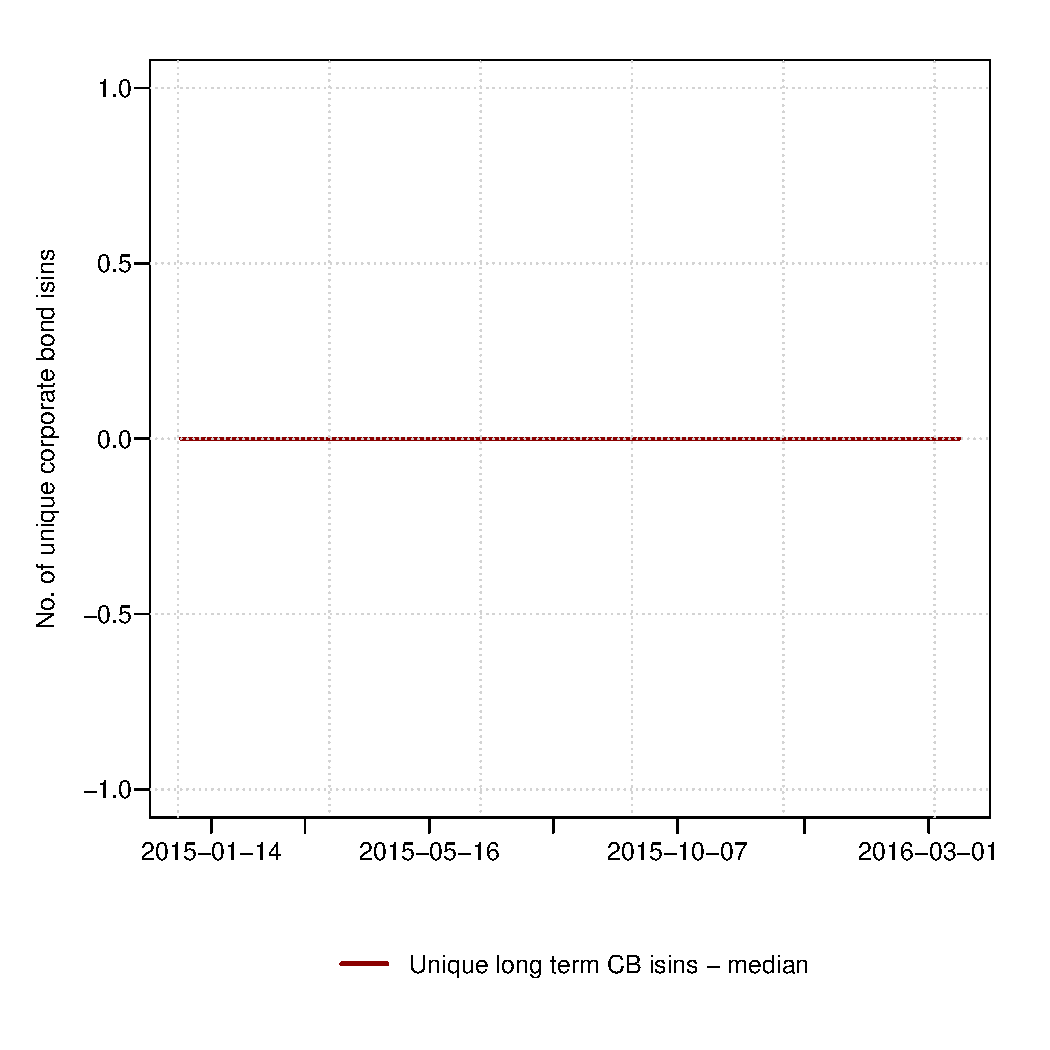
\includegraphics[width=0.8\paperwidth,height=0.5\paperwidth]{../GRAPHS/fpi_median_st_cbs_all.pdf}     %
% \end{frame}                                                                                              %
%                                                                                                          %
% \begin{frame}                                                                                            %
%  \frametitle{Unique commercial papers ISINs - Median}                                                    %
%    \centering                                                                                            %
%    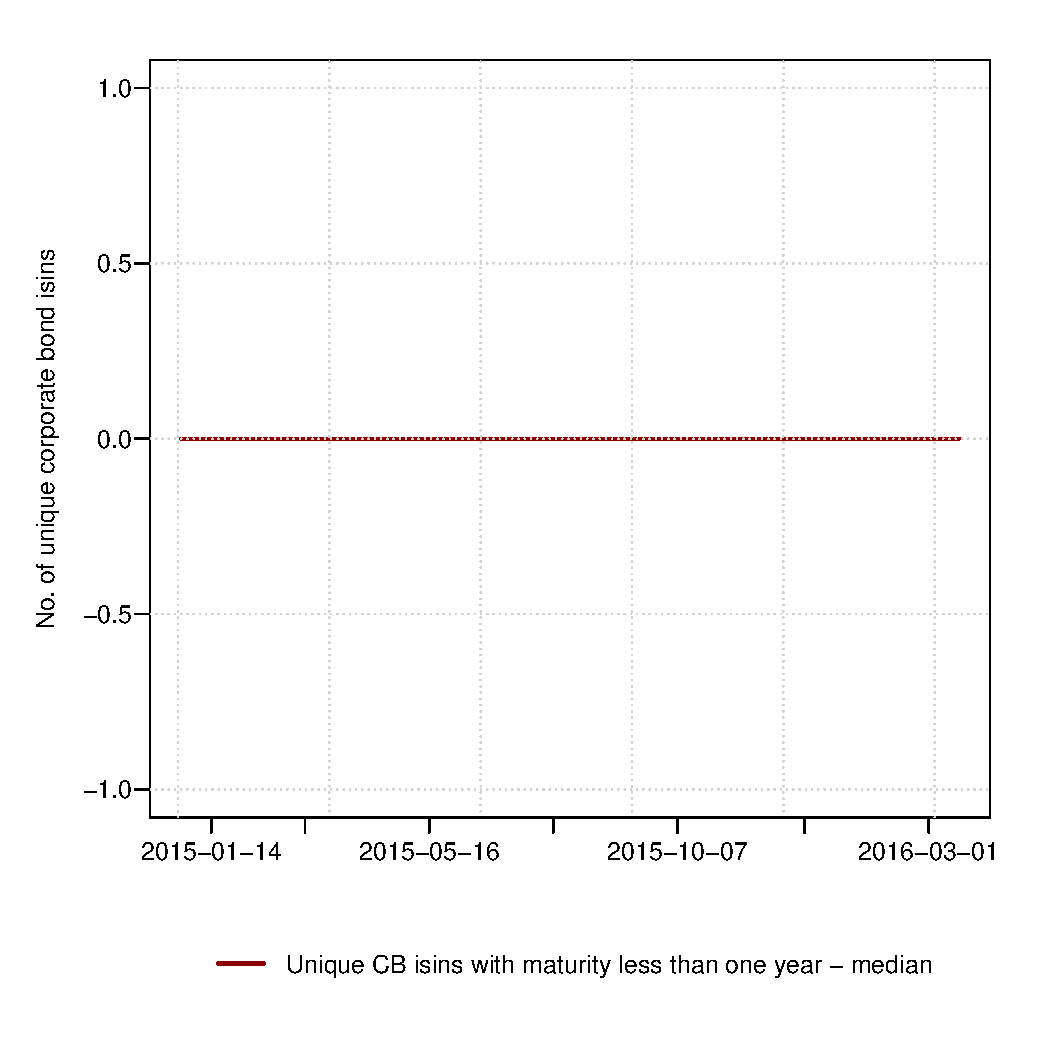
\includegraphics[width=0.8\paperwidth,height=0.5\paperwidth]{../GRAPHS/fpi_median_one_yr_cbs_all.pdf} %
% \end{frame}                                                                                              %
%%%%%%%%%%%%%%%%%%%%%%%%%%%%%%%%%%%%%%%%%%%%%%%%%%%%%%%%%%%%%%%%%%%%%%%%%%%%%%%%%%%%%%%%%%%%%%%%%%%%%%%%%%%%

\begin{frame}
\frametitle{Outstanding bond holdings as 02-02-2015}
\begin{table}[ht]
\centering
\begin{tabular}{rccc}
  \hline
  & Long term & Short term & CPs  \\  
  \hline
  Total & 527,041,743 & 388676 & 33900 \\    
  FPI & 51,920,391 & 89,492 & 0 \\
  \hline
\end{tabular}
\end{table}

\begin{itemize}
  \item About 9.9\% of total long term corporate bonds and 23\% of total short
    term corporate bonds are held by FPIs.
\end{itemize}
\end{frame}


\begin{frame}
\frametitle{Monthly portfolio composition of FPIs}
\begin{table}[ht]
\centering
\begin{tabular}{cccccc}
  \hline
  Date & Long term (\%)& Short term (\%) & CPs (\%) & Equity (\%)  & Others (\%) \\  
  \hline
  2015-01-31 & 0.10 & 0.00011 & 0 & 96.20 & 3.70 \\ 
  2015-02-28 & 0.10 & 0.00011 & 0 & 96.21 & 3.69 \\ 
  2015-03-31 & 1.30 & 0.00011 & 0 & 96.14 & 3.76 \\ 
  2015-04-29 & 0.93 & 0.00011 & 0 & 96.22 & 3.68 \\ 
  2015-05-30 & 0.89 & 0.00011 & 0 & 96.11 & 3.78 \\ 
  2015-06-30 & 0.92 & 0.00010 & 0 & 96.13 & 3.76 \\ 
  2015-07-31 & 0.86 & 0.00010 & 0 & 96.12 & 3.76 \\ 
  2015-08-29 & 0.87 & 0.00010 & 0 & 96.05 & 3.82 \\ 
  2015-09-30 & 0.81 & 0.00010 & 0 & 95.55 & 4.32 \\ 
  2015-10-31 & 0.78 & 0.00011 & 0 & 95.99 & 3.88 \\ 
  2015-11-28 & 0.79 & 0.00011 & 0 & 96.17 & 3.68 \\ 
  2015-12-30 & 0.81 & 0.00010 & 0 & 95.55 & 4.32 \\ 
  2016-01-30 & 0.80 & 0.00010 & 0 & 95.53 & 4.34 \\ 
  2016-02-27 & 0.79 & 0.00010 & 0 & 95.34 & 4.52 \\ 
  2016-03-18 & 0.81 & 0.00009 & 0 & 95.46 & 4.38 \\ 
  \hline
\end{tabular}
\end{table}

\end{frame}



\begin{frame}
 \frametitle{Total FPI corporate bond holdings}
   \centering
   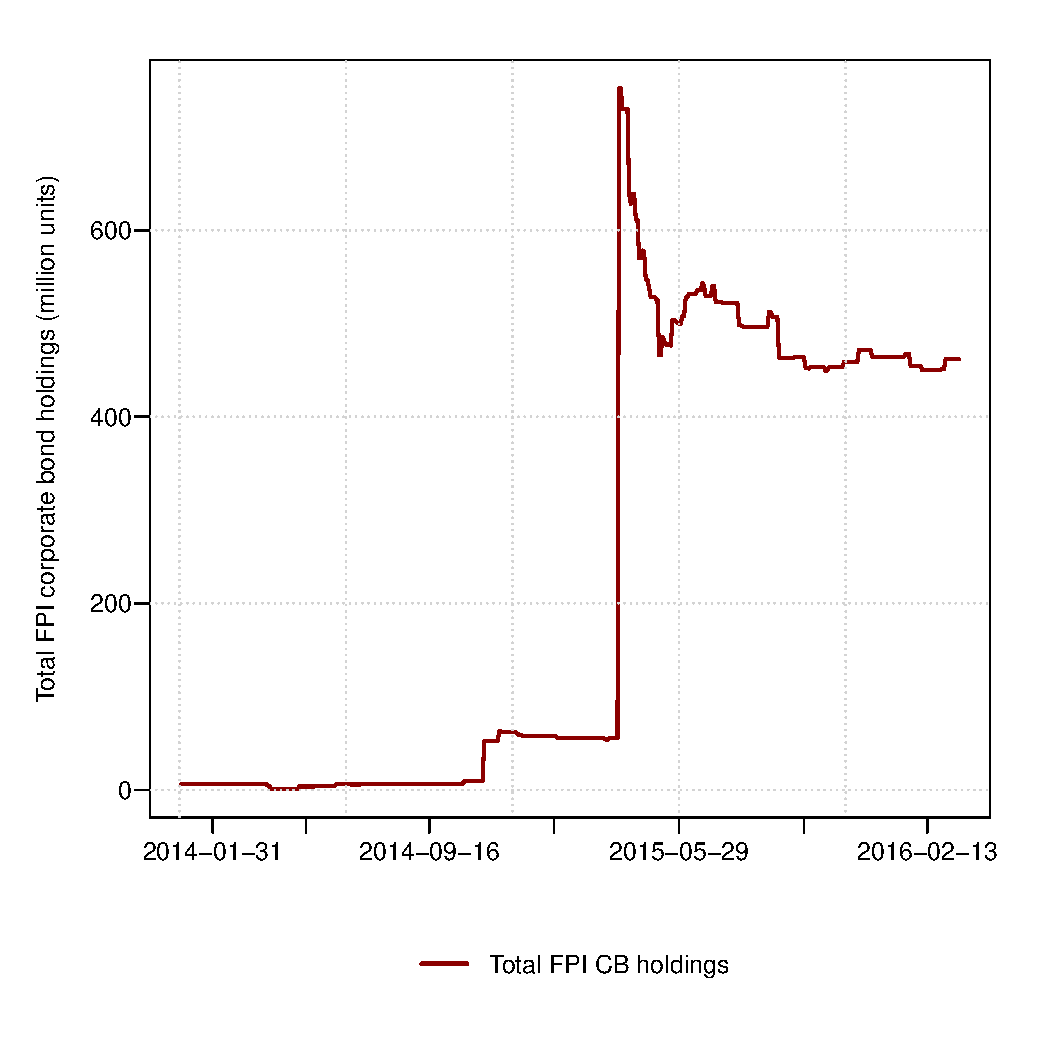
\includegraphics[width=0.8\paperwidth,height=0.5\paperwidth]{../GRAPHS/fpi_sum_all_cbs_all.pdf}
\end{frame}


\begin{frame}
 \frametitle{Total FPI long term corporate bond holdings}
   \centering
   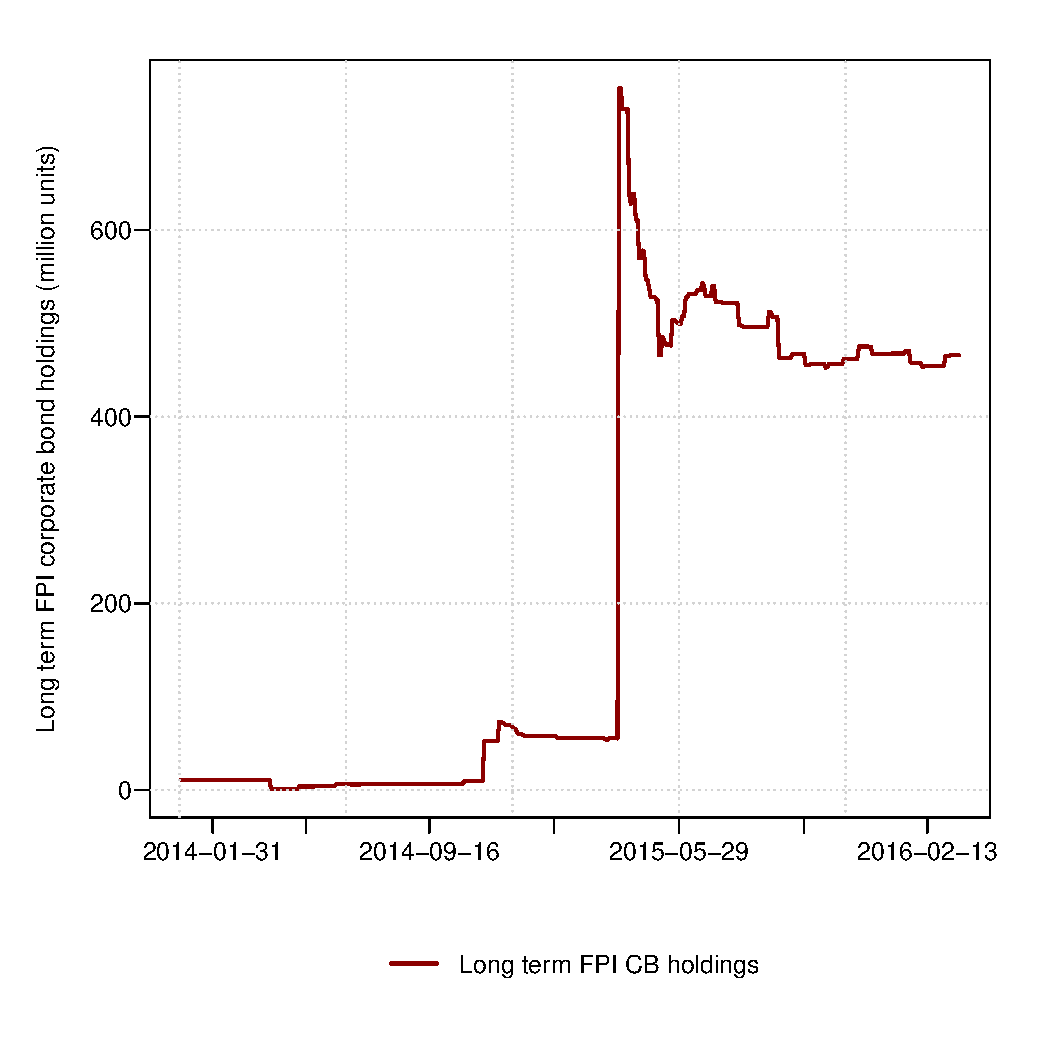
\includegraphics[width=0.8\paperwidth,height=0.5\paperwidth]{../GRAPHS/fpi_sum_long_term_cbs_all.pdf}
\end{frame}

\begin{frame}
 \frametitle{Total FPI long term corporate bond holdings- barring NTPC}
   \centering
   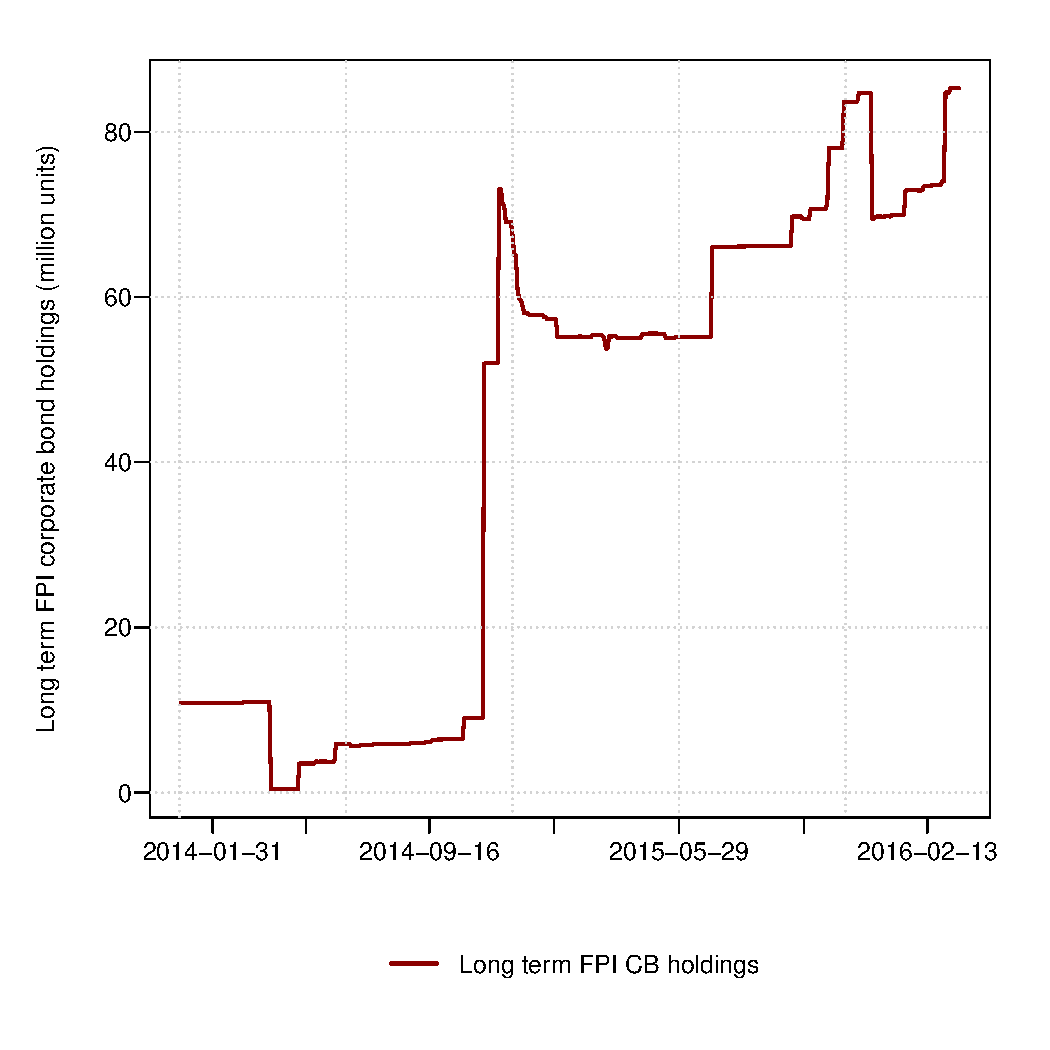
\includegraphics[width=0.8\paperwidth,height=0.5\paperwidth]{../GRAPHS/fpi_sum_long_term_minus_ntpc_cbs_all.pdf}
\end{frame}

\begin{frame}
 \frametitle{Proportion of FPIs in long term corporate bonds}
   \centering
   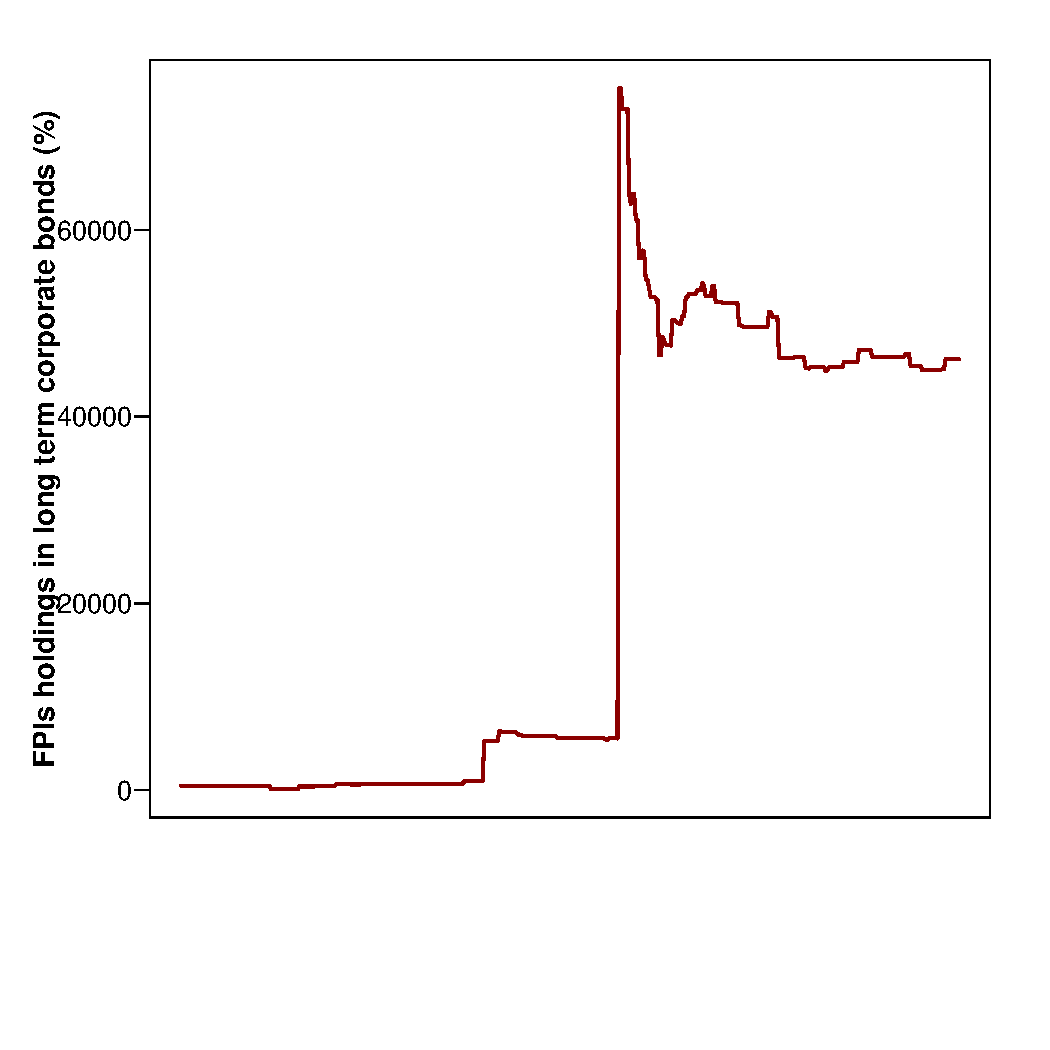
\includegraphics[width=0.8\paperwidth,height=0.5\paperwidth]{../GRAPHS/fpi_sum_long_term_prop.pdf}
\end{frame}



\begin{frame}
 \frametitle{Total FPI short term corporate bond holdings}
   \centering
   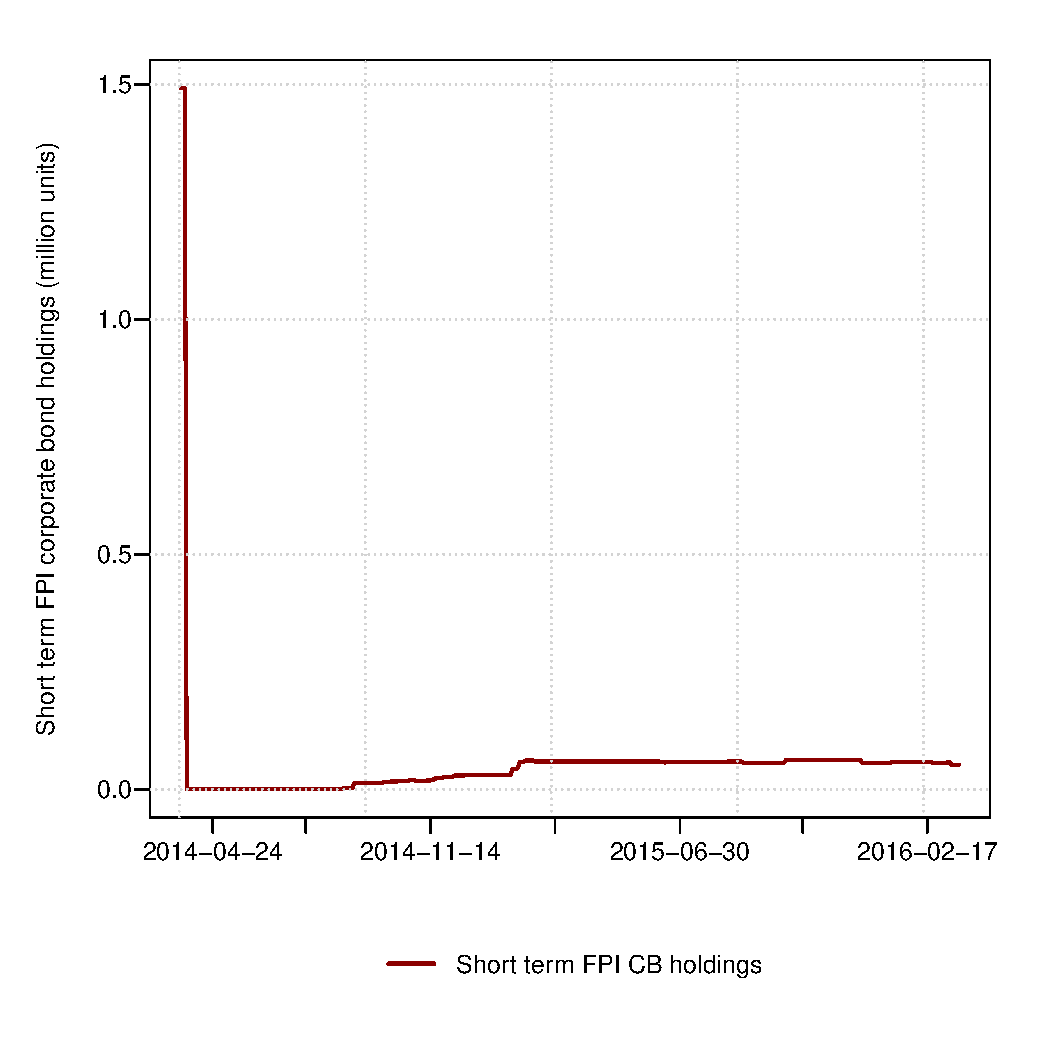
\includegraphics[width=0.8\paperwidth,height=0.5\paperwidth]{../GRAPHS/fpi_sum_short_term_cbs_all.pdf}
\end{frame}

% \begin{frame}
%  \frametitle{Proportion of FPIs in short term corporate bonds}
%    \centering
%    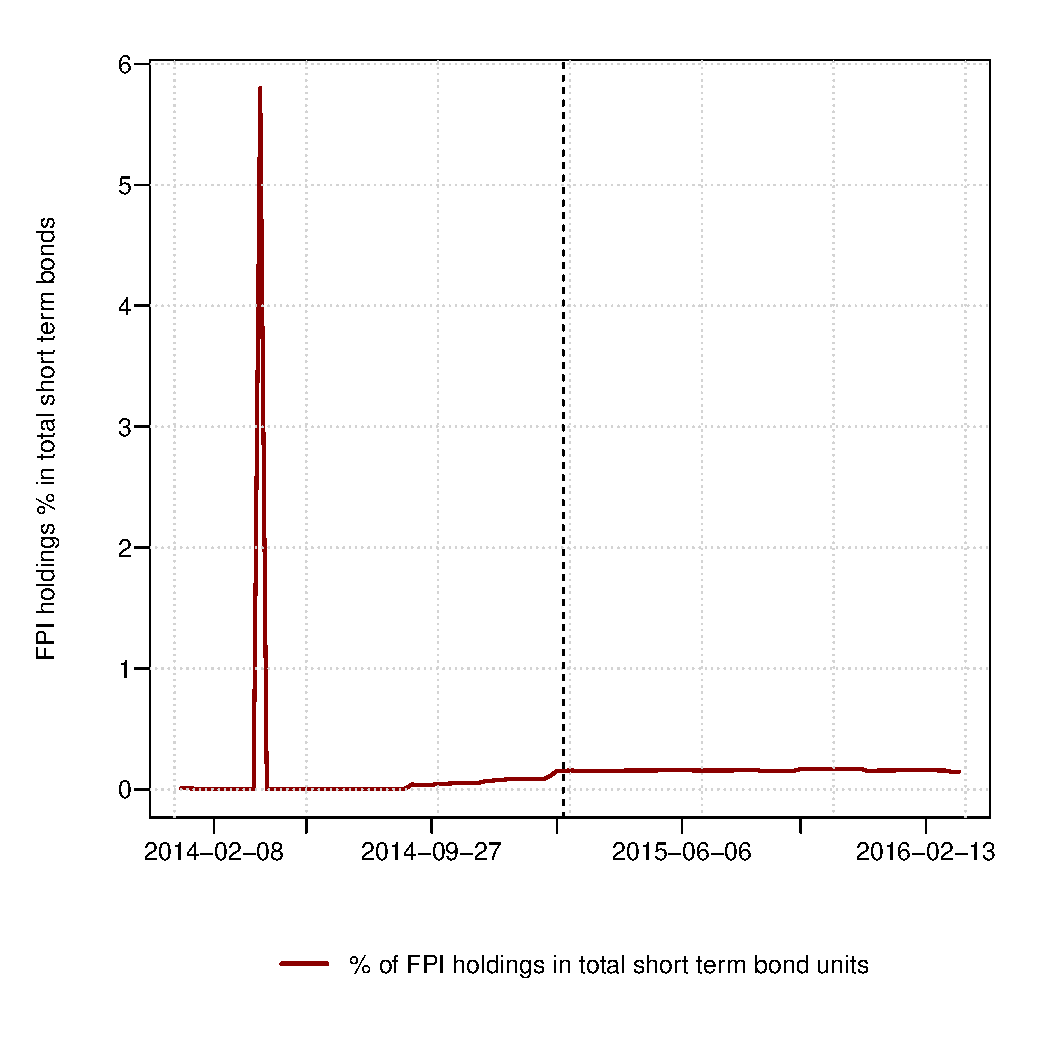
\includegraphics[width=0.8\paperwidth,height=0.5\paperwidth]{../GRAPHS/fpi_sum_short_term_prop.pdf}
% \end{frame}


% \begin{frame}
%  \frametitle{Total FPI commercial paper holdings}
%    \centering
%    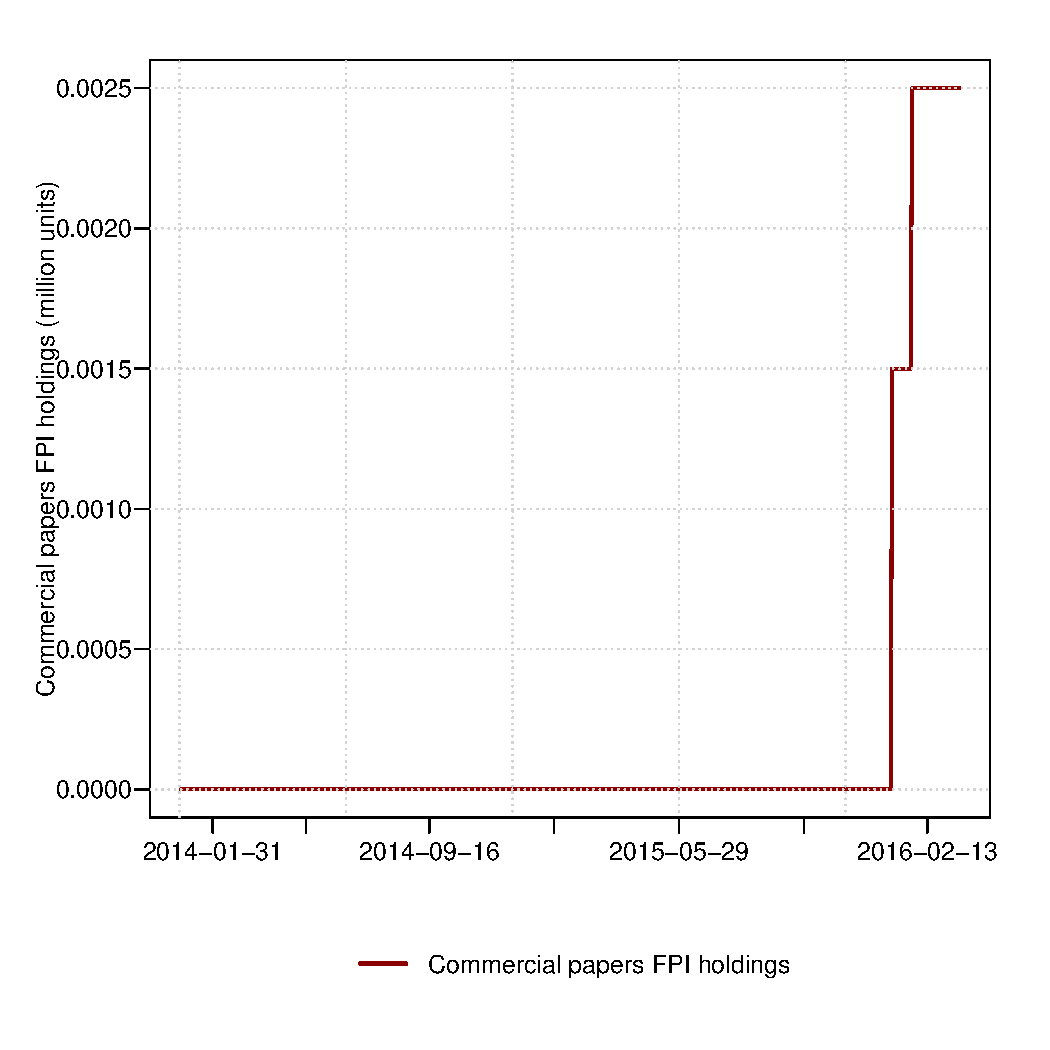
\includegraphics[width=0.8\paperwidth,height=0.5\paperwidth]{../GRAPHS/fpi_sum_commercial_paper_cbs_all.pdf}
% \end{frame}

\begin{frame}
 \frametitle{Total FPI equity holdings}
   \centering
   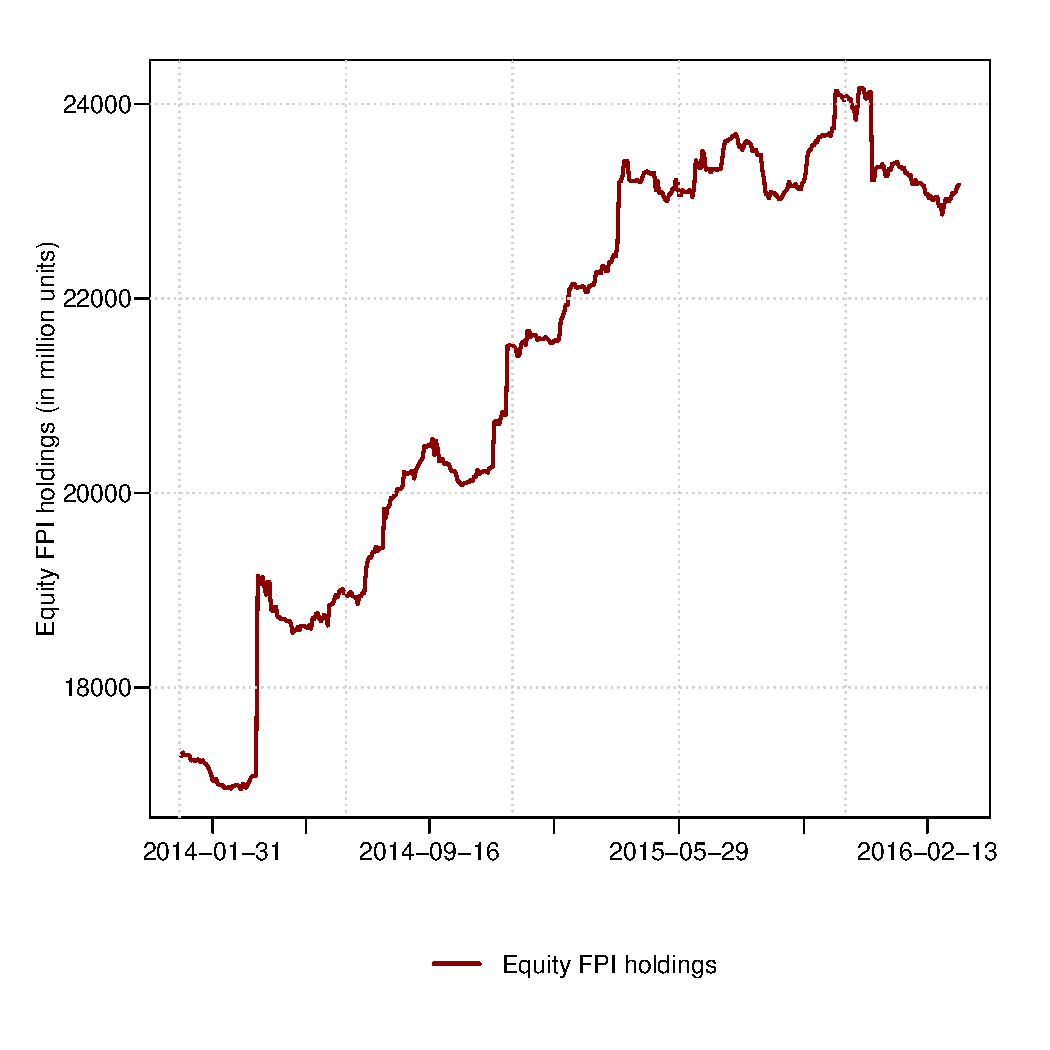
\includegraphics[width=0.8\paperwidth,height=0.5\paperwidth]{../GRAPHS/fpi_sum_equity_all.pdf}
\end{frame}



\section{comments}

\begin{frame}

  \begin{center}
    Questions/comments?
  \end{center}
\end{frame}
 
\end{document}
 

%%% Local Variables:
%%% mode: latex
%%% TeX-master: t
%%% End:


